\begin{center}
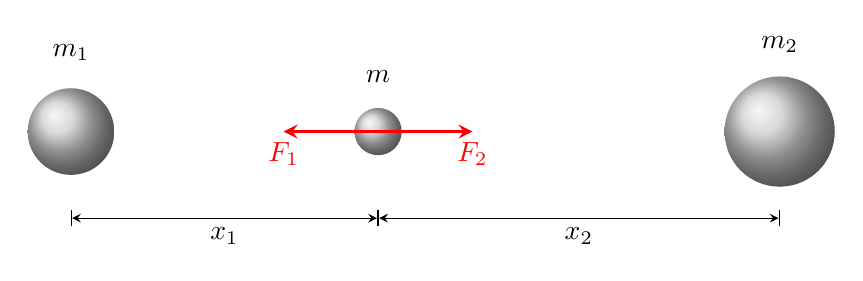
\begin{tikzpicture}[>=stealth]
 \shade[ball color=gray!40] (0,0) circle (0.55);
 \shade[ball color=gray!40] (9,0) circle (0.7);
 \shade[ball color=gray!40] (3.9,0) circle (0.3);
 \node at (0,1.0) {$m_1$};
 \node at (9,1.1) {$m_2$};
 \node at (3.9,0.7) {$m$};
 \draw[->, very thick, red] (3.9,0) -- (2.7,0) node[below] {$F_1$};
 \draw[->, very thick, red] (3.9,0) -- (5.1,0) node[below] {$F_2$};
 \draw[|<->|] (0,-1.1) -- (3.9,-1.1) node[midway, below] {$x_1$};
 \draw[|<->|] (3.9,-1.1) -- (9,-1.1) node[midway, below] {$x_2$};
\end{tikzpicture}
\end{center}

Die Kugel mit der Masse $m$ ist im Gleichgewicht, wenn die beiden Gravitationskräfte gleich gross sind:
\begin{align}
 G\,\frac{m_1\,m}{x_1^2} &= G\,\frac{m_2\,m}{x_2^2}
 \quad\Rightarrow\quad \frac{x_1^2}{x_2^2} = \frac{m_1}{m_2}
\end{align}
Die Masse $m$ und die Gravitationskonstante fallen heraus. Mit $m_1 = \mEiO$ und $m_2 = \mZwO$:
\begin{align}
 \frac{x_1}{x_2} &= \vhF = \sqrt{\frac{\mEi}{\mZw}} = \frac{\sqrt{3}}{\sqrt{5}} = \vh \approx \result{\vhP{0}{2}}
\end{align}
Die Kugel liegt näher bei der leichteren Kugel, nämlich beim Bruchteil
\begin{align}
 \frac{x_1}{x_1+x_2} &= \antF = \ant \approx \antP{0}{2}
\end{align}
des Abstands, von der Kugel mit \mEiO\ aus gemessen.
